\documentclass[titlepage,a4paper,12pt,AutoFakeBold]{article}
%\NeedsTeXFormat{LaTeX2e}[2005/12/01]
\usepackage{xeCJK}
\setCJKmainfont{SimSun}
%\usepackage[margin=1in]{geometry}
\usepackage{geometry}
\geometry{a4paper,left=3.18cm,right=3.18cm,top=2.54cm,bottom=2.54cm}
\usepackage{braket}
\usepackage{graphicx}


\usepackage[hidelinks]{hyperref}
\hypersetup{
%linkbordercolor={1 1 1},
urlcolor=blue,
}
\usepackage{float}
\usepackage[bottom]{footmisc}

\usepackage{algorithm}
\usepackage[noend]{algpseudocode}
%\usepackage{longtable}
\usepackage{amsmath}
\usepackage{amssymb}
\usepackage{extarrows}
%\usepackage{tabularx}
%\usepackage{rotating}
\usepackage {indentfirst}
\usepackage{courier}
\usepackage[dvipsnames]{xcolor}
\usepackage{listings}
%\usepackage{xcolor}\lstset{}
\lstset{
	basicstyle={\sffamily\footnotesize},
	%	numbers=left,
	%	numberstyle=\tiny\color{gray},
	numbersep=5pt,
	breaklines=true,
	captionpos={T},
	frame={lines},
%%	rulecolor=,
	framerule=0.5pt,
	columns=flexible,
	tabsize=2,
	numbers=left,
%	backgroundcolor = \color{White},
	backgroundcolor={\color{yellow!3!white}}
%	language=Mathematica,
%	keywordstyle=\color{black}
}
\usepackage{enumitem}
%\allowdisplaybreaks[4]
%\usepackage{mathematica}
%\definecolor{darkred}{rgb}{0.5 0 0}
%\definecolor{darkgreen}{rgb}{0.5 .5 0}
%\definecolor{darkblue}{rgb}{0 0 .5}



%\usepackage{listings}
%\renewcommand{\lstlistingname}{Listing}


%\renewcommand{\contentsname}{目录}
\newcommand\litem[1]{\item{ #1?\\}}
%\newcommand{\dollar}{\mbox{\textdollar}} \bfseries

\makeatletter

\makeatother






\begin{document}



\title{\textsf{MagneticTB} manual}
%\vtitle{利用群表示理论研究三维晶体中的演生粒子}
%\author{张泽英}
\author{Zeying Zhang}

\maketitle

%\newpage

\tableofcontents

\newpage

\section{Features}
\textsf{MagneticTB} is an open-source software package developed based on the co-representation theory of magnetic groups. It can generate tight-binding models that satisfy any of the 1651 magnetic group symmetries. The specific features are as follows:
\begin{itemize}
\item   The corresponding tight-binding model can be constructed simply by inputting the magnetic group number and the information of each Wyckoff position.
\item	Obtain the symmetry operations of the 1651 magnetic groups.
\item	Interface with other software.
\item	Plot the energy spectrum, and the spectrum can be dynamically displayed with changes in the parameters.
\item	Construct tight-binding models of non-magnetic materials.
\item	Consider non-collinear magnetic structures.
\item	Construct tight-binding models of single groups (without spin) and magnetic double groups (with spin).
\end{itemize}


\section{Installation}

First, log in to the homepage of the \textsf{MagneticTB} package on GitHub (no account or password required):
\begin{center}
\url{https://github.com/zhangzeyingvv/MagneticTB}
\end{center}
Click "Code", "Download ZIP", and download the MagneticTB-main.zip file, as shown in the following figure:
\begin{figure}[h]
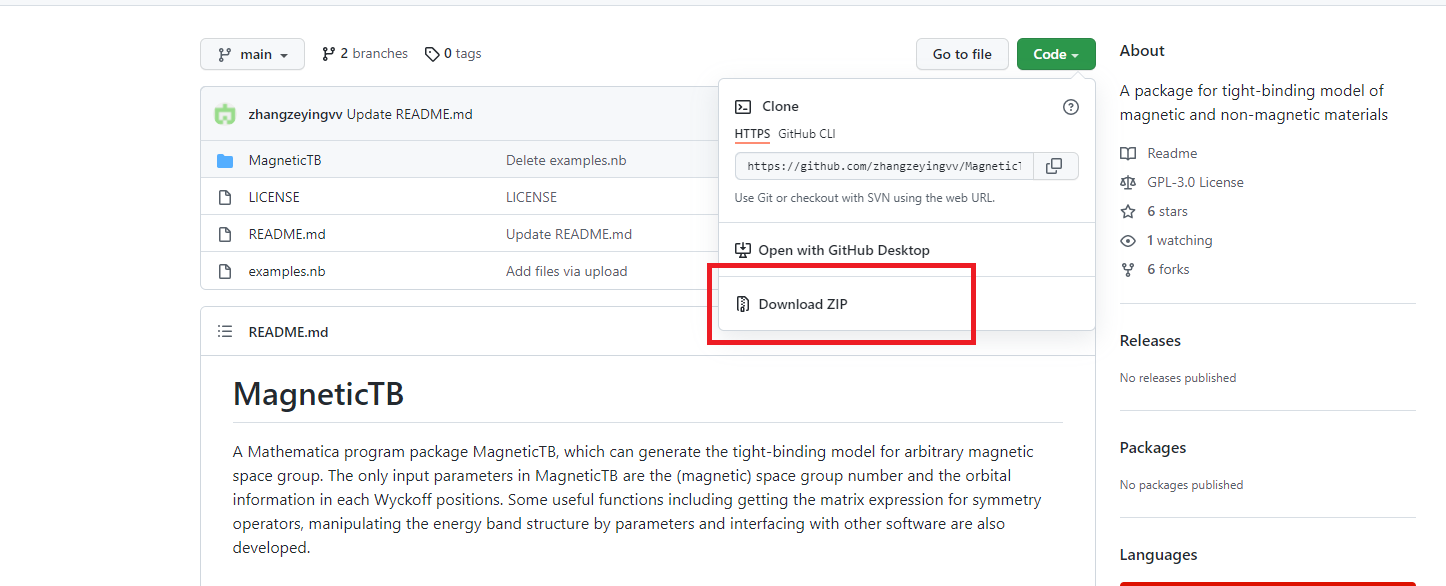
\includegraphics[width=1\textwidth]{./figures/安装1}
\end{figure}


Open Mathematica and run:
\begin{lstlisting}[numbers=none]
$UserBaseDirectory
\end{lstlisting}
%\lstinline| $\mbox{\$}$ |
Click Shift+Enter to run. Open the displayed directory and go to the "Applications" folder.

Unzip the previously downloaded MagneticTB-main.zip file to get a MagneticTB folder and three files. Copy the unzipped MagneticTB folder to the "Applications" folder to complete the installation. Run in Mathematica:
\begin{lstlisting}[numbers=none]
Needs["MagneticTB`"]
\end{lstlisting}	
The package can be loaded by running the above command. Experienced users can install it anywhere in the \lstinline|$Path|, but some directories may require administrator privileges. The above method is applicable to both Windows and Linux users. For more information, please refer to Comput. Phys. Commun., 270, 108153 (2022).

\section{Capabilities of MagneticTB}
\subsection{Core module}
The core functionality of \textsf{MagneticTB} is to construct symmetry-adapted tight-binding models, consisting of three main functions: \lstinline|msgop|, \lstinline|init|, and \lstinline|symham|.

\lstinline|msgop| can provide the symmetry operations for any of the 1651 magnetic groups, for example:
\begin{lstlisting}
msgop[gray[191]]
msgop[bnsdict[{191, 236}]]
msgop[ogdict[{191, 8, 1470}]]
\end{lstlisting}	
In the first line, \lstinline|gray[191]| obtains the code for the gray group with number 191 (which is the space group with time-reversal symmetry);
In the second line, \lstinline|bnsdict[{191, 236}]| obtains the code for the magnetic group with BNS number $191.236$;
In the third line, \lstinline|ogdict[{191, 8, 1470}]| obtains the code for the magnetic group with OG number $191.8.1470$.

Using \lstinline|msgop[code]| gives the symmetry operations for the corresponding magnetic group. The above three commands are actually equivalent, and their output is:

\begin{lstlisting}
Magnetic space group (BNS): {191.234,P6/mmm1'}
Lattice: HexagonalP
Primitive Lattice Vactor: {{a,0,0},{-(a/2),(Sqrt[3] a)/2,0},{0,0,c}}
Conventional Lattice Vactor: {{a,0,0},{-(a/2),(Sqrt[3] a)/2,0},{0,0,c}}

{{"1",{{1,0,0},{0,1,0},{0,0,1}},{0,0,0},F},
{"6z",{{1,-1,0},{1,0,0},{0,0,1}},{0,0,0},F},
{"3z",{{0,-1,0},{1,-1,0},{0,0,1}},{0,0,0},F},
...
{"1",{{1,0,0},{0,1,0},{0,0,1}},{0,0,0},T},
{"6z",{{1,-1,0},{1,0,0},{0,0,1}},{0,0,0},T},
{"3z",{{0,-1,0},{1,-1,0},{0,0,1}},{0,0,0},T},
...}
\end{lstlisting}
Lines 1-4 show the basic information of the magnetic group, including its symbol, lattice type, and lattice vectors. Lines 6-13 show the symmetry operations for the gray group with number 191, where the first four columns correspond to the name of the symmetry operation, its rotation part, its translation part, and whether it includes time-reversal operation.

With the symmetry operations, we can use the \lstinline|init| function to initialize the structure:
\begin{lstlisting}
sgop=msgop[gray[191]];
init[
	lattice -> {{a, 0, 0}, {-(a/2), (Sqrt[3] a)/2, 0}, {0, 0, c}},
	lattpar -> {a -> 1, c -> 3},
	wyckoffposition -> {{{1/3, 2/3, 0}, {0, 0, 0}}},
	symminformation -> sgop,
	basisFunctions -> {{"pz"}}];
\end{lstlisting}	
The \lstinline|init| function has five options that must be set. The \lstinline|lattice| option corresponds to lattice vectors and the \lstinline|symminformation| option corresponds to the set of symmetry operations, which can directly use the output of \lstinline|msgop| as the option value or use user-defined symmetry operations. The \lstinline|lattpar| option corresponds to the numerical values of the lattice vectors parameters, and the \lstinline|wyckoffposition| option corresponds to the Wyckoff positions to be considered. Its format is:
\[
\{\{\boldsymbol{a}_{1},\boldsymbol{m}_{1}\},\{\boldsymbol{a}_{2},\boldsymbol{m}_{2}\},...\}
\]
The $\boldsymbol{a}{i}$ and $\boldsymbol{m}{i}$ in the above text refer to the coordinates and magnetization directions of the $i$th Wyckoff position. For equivalent Wyckoff positions, only one of them needs to be input.

The \lstinline|basisFunctions| option specifies the basis functions to be considered for each Wyckoff position. The format is:
\[
\{b_{1},b_{2},...\}
\]
$b_{i}$ is the list of basis functions to be considered for the $i$th Wyckoff point.
The correspondence between basis functions and strings is shown in the following table:
\begin{table}[H]
	\centering 
%\caption{\lstinline!basisFunctions!中原子轨道和字符串的对应关系}
	\label{tab:bf} %
	\begin{tabular}{cc|cc}
		\hline 
		basis function & code  & basis function  & code \tabularnewline
		\hline 
		$s$  & \lstinline!"s"! & $p_{x}$  & \lstinline!"px"! \tabularnewline
		\hline 
		$p_{y}$  & \lstinline!"py"! & $p_{z}$  & \lstinline!"pz"! \tabularnewline
		\hline 
		$p_{x}+ip_{y}$  & \lstinline!"px+ipy"! & $p_{x}-ip_{y}$  & \lstinline!"px-ipy"! \tabularnewline
		\hline 
		$d_{z^{2}}$  & \lstinline!"dz2"! & $d_{xy}$  & \lstinline!"dxy"! \tabularnewline
		\hline 
		$d_{yz}$  & \lstinline!"dyz"! & $d_{xz}$  & \lstinline!"dxz"! \tabularnewline
		\hline 
		$d_{x^{2}-y^{2}}$  & \lstinline!"dx2-y2"!  &  & \tabularnewline
		\hline 
	\end{tabular}
\end{table}
To include spin, simply add \lstinline!"up"! or \lstinline!"dn"! after the basis function name, for example, \lstinline!{"pzup","dxydn"}!. If a basis function is not listed in the above table, one can input its analytic expression directly. For example, if one wants to include the $f_{xyz}$ orbital, they can input \lstinline!basisFunctions -> {{x*y*z}}!.

To check if the generated structure is correct after running the initialization function, you can use the \lstinline|atompos| function.
\begin{lstlisting}
In:= atompos
Out:= {{{{1/3, 2/3, 0}, {0, 0, 0}}, {{2/3, 1/3, 0}, {0, 0, 0}}}}
\end{lstlisting}
It indicates that there are two atomic positions to be considered in the primitive cell of the structure, which are $(1/3,2/3,0)$ and $(2/3,1/3,0)$. The magnetic moment of both atoms is \lstinline|{0, 0, 0}|, indicating that they are nonmagnetic. After running \lstinline!init!, the basic properties that can be obtained are shown in the following table:

\begin{table}[ht]
	\centering
	% \caption{}
	\label{tab:pro} %
	\begin{tabular}{c|c}
		\hline
		code & properties \tabularnewline
		\hline
		\lstinline!atompos! & The atomic coordinates and magnetic directions for each atom \tabularnewline
		\hline
		\lstinline!wcc! & Atom position of each orbital \tabularnewline
		\hline
		\lstinline!reclatt! & Reciprocal lattice vector \tabularnewline
		\hline
		\lstinline!symmetryops! & Representation matrix for symmetry operators \tabularnewline
		\hline
		\lstinline!unsymham[n]! & Generating the Hamiltonian without any symmetry constraints \tabularnewline
		\hline
		\lstinline!symham[n]! & Generating the Hamiltonian with symmetry constraints \tabularnewline
		\hline
		\lstinline!symmcompile! & Information about symmetry operations and representation matrices \tabularnewline
		\hline
		\lstinline!bondclassify! & Provides bond lengths for all neighbors \tabularnewline
		\hline
		\lstinline!showbonds[n]! & Show bond lengths for $(n-1)$th nearest neighbors \tabularnewline
		\hline
	\end{tabular}
\end{table}

After verifying the accuracy of the information, \lstinline|symham[n]| can be used to generate a symmetrized tight-binding Hamiltonian considering the $(n-1)$th nearest neighbors. For example,
\begin{lstlisting}[numbers=none]
	symham[1]
\end{lstlisting}
will generate the Hamiltonian with only on-site energies, while
\begin{lstlisting}[numbers=none]
	Sum[symham[n], {n, 1, 3}];
\end{lstlisting}
will generate the Hamiltonian considering on-site energies, nearest and next-nearest neighbor interactions.

\subsection{Plotting module}
There are two functions in the plotting module, \lstinline|bandplot| and \lstinline|bandManipulate|. Usage is as follows:
\begin{lstlisting}[numbers=none]
	bandplot[band path, number of points in each segment, symham-generated Hamiltonian, parameter values]
	bandManipulate[band path, number of points in each segment, symham-generated Hamiltonian]
\end{lstlisting}
\lstinline|bandplot| can generate a beautiful band plot, which can be directly used as a figure in a paper. \lstinline|bandManipulate| can generate a dynamic band plot that changes with the parameter values. See example in \ref{gra}.

\subsection{Interface module}
The interface module can convert the Hamiltonian generated by \lstinline|symham| into the wannier90\_hr.dat file format. Usage is as follows:
\begin{lstlisting}[numbers=none]
	hop[symham-generated Hamiltonian, parameter values]
\end{lstlisting}
See example in \ref{gra}. Note that the Hamiltonian generated by \lstinline|symham| should be used as input. \textbf{Do not use the Hamiltonian resolved by yourself as input. If you want certain parameters to be zero, specify them as zero in the parameter values.}

\section{Example}
\subsection{Graphene}
\label{gra}
To generate the tight-binding model of graphene near the Fermi surface, one only needs to know the $2c$ Wyckoff point of two carbon atoms in the 191st space group and that the electronic states near the Fermi surface are composed of carbon atoms' $p_z$ orbitals.
% Use \textsf{MagneticTB} to construct the tight-binding model.
The specific code is as follows:
\begin{lstlisting}
	Needs["MagneticTB`"];
	sgop = msgop[gray[191]];
	init[
	lattice -> {{a, 0, 0}, {-(a/2), (Sqrt[3] a)/2, 0}, {0, 0, c}},
	lattpar -> {a -> 1, c -> 3},
	wyckoffposition -> {{{1/3, 2/3, 0}, {0, 0, 0}}},
	symminformation -> sgop,
	basisFunctions -> {{"pz"}}];
	ham = Sum[symham[i], {i, 3}];
	MatrixForm[ham]
\end{lstlisting}
The first line loads the \textsf{MagneticTB} package. The second line gets the symmetry operations of the 191st gray space group. The third line is the initialization function. The fourth to eighth lines are the parameters of the initialization function. The fourth line is the lattice vector. The fifth line is the value of the parameters in the lattice constant. The sixth line is the Wyckoff point coordinates and magnetic direction to be considered. The seventh line is the symmetry satisfied by the symmetrized tight-binding model. The eighth line is the atomic orbitals to be considered. The ninth line is the output Hamiltonian including the next-nearest neighbor.

To consider spin-orbit coupling, simply change the 8th line of the code from:

\begin{lstlisting}[numbers=none]
	basisFunctions -> {{"pz"}}];
\end{lstlisting}

to:

\begin{lstlisting}[numbers=none]
	basisFunctions -> {{"pzup","pzdn"}}];
\end{lstlisting}

Then,

\begin{lstlisting}[numbers=none]
	sgop = msgop[gray[191]];
	init[lattice -> {{a, 0, 0}, {-(a/2), (Sqrt[3] a)/2, 0}, {0, 0, c}},
	lattpar -> {a -> 1, c -> 3},
	wyckoffposition -> {{{1/3, 2/3, 0}, {0, 0, 0}}},
	symminformation -> sgop,
	basisFunctions -> {{"pzup", "pzdn"}}];
	hamsoc = Sum[symham[i], {i, 3}];
	MatrixForm[hamsoc]
\end{lstlisting}

will generate the Hamiltonian that includes spin-orbit coupling. Once the Hamiltonian is obtained, band structures can be plotted and wannier90\_hr.dat can be generated. The specific code for plotting the band structure is as follows:
\begin{lstlisting}
	path={
		{{{0,0,0},{0,1/2,0}},{"G","M"}},
		{{{0,1/2,0},{1/3,1/3,0}},{"M","K"}},
		{{{1/3,1/3,0},{0,0,0}},{"K","G"}}
	};
	bandManipulate[path, 20, ham]
	bandplot[path, 200, ham, {e1 −> 0.05, t1 −> 0.5, r1−> 0}]
\end{lstlisting}
The first five lines define the $\boldsymbol{k}$-point path, the sixth line dynamically displays the band structure, and the seventh line plots the band structure for the given parameters. The results are shown in the following figure:
\begin{figure}[H]
	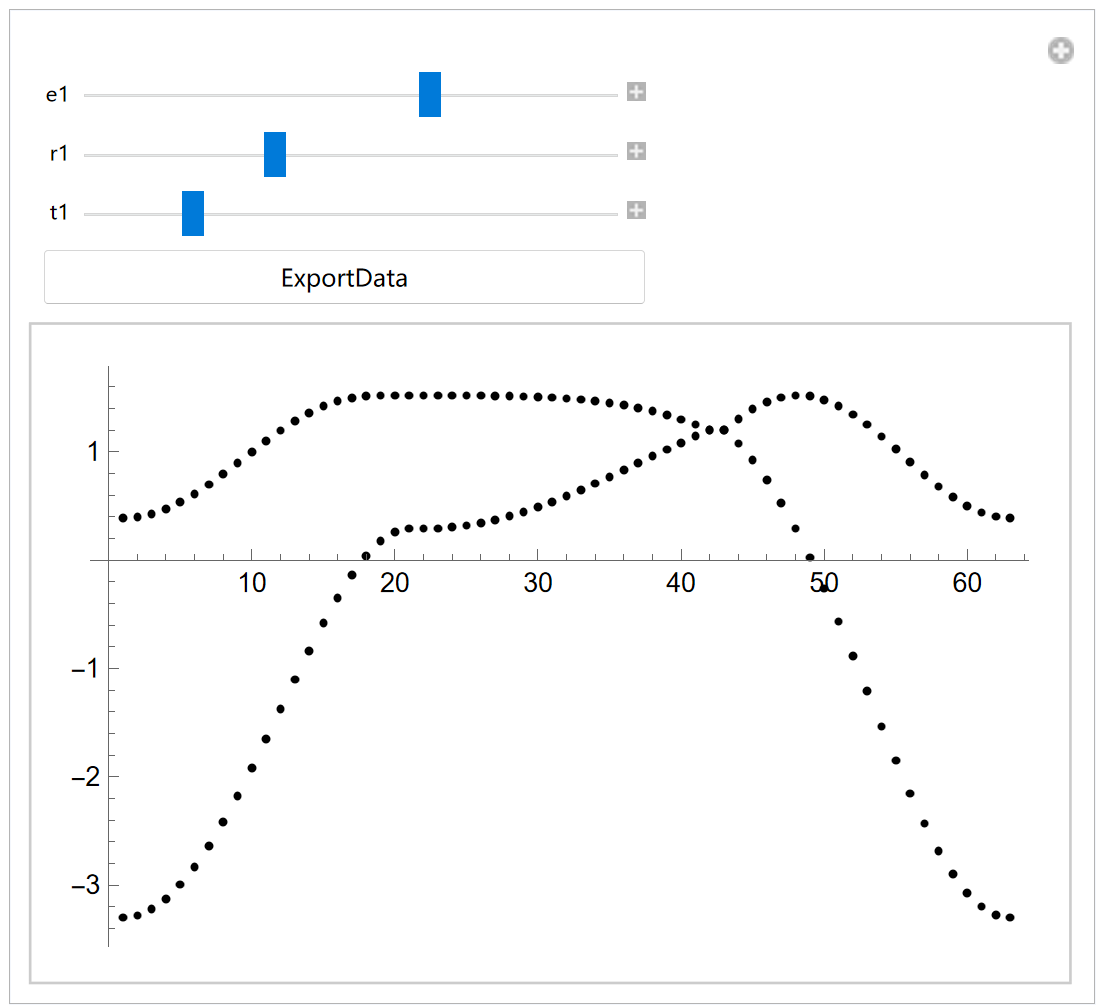
\includegraphics[width=.45\textwidth]{./figures/bm}
	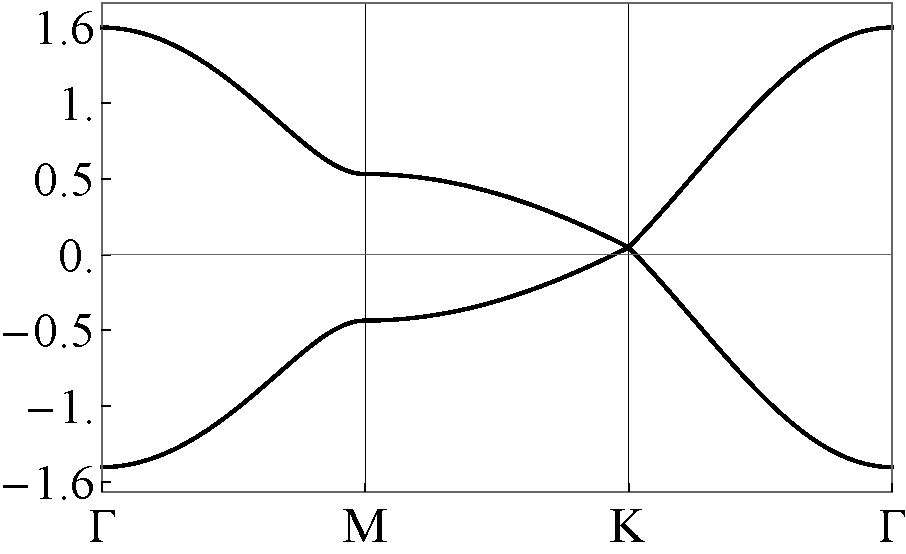
\includegraphics[width=.54\textwidth]{./figures/grabd}
\end{figure}
\noindent Clicking on "ExportData" displays the size of the parameters.

The command \lstinline|showbonds| can be used to display the bond lengths between neighboring atoms in graphene. For example, to display the bond lengths for the next-nearest neighbors, use \lstinline|showbonds[3]|. The output is shown below:
\begin{center}
	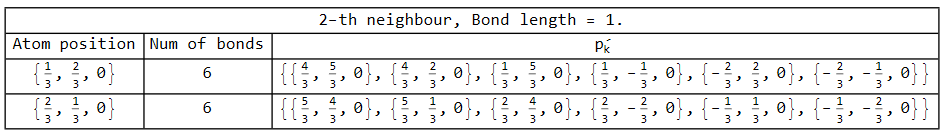
\includegraphics[width=1.0\textwidth]{./figures/showbonds.png}
\end{center}

To generate the wannier90\_hr.dat file, simply run the following command:
\begin{lstlisting}[numbers=none]
	hop[ham, {e1 -> 0, r1 -> 0.02, t1 -> 0.5}]
\end{lstlisting}
The result is:
\begin{lstlisting}[numbers=none]
	Generated by MagneticTB
	2
	7
	1    1    1    1    1    1    1
	-1    -1     0     1     1    0.02000000    0.00000000
	-1    -1     0     2     1    0.00000000    0.00000000
	-1    -1     0     1     2    0.00000000    0.00000000
	-1    -1     0     2     2    0.02000000    0.00000000
	-1     0     0     1     1    0.02000000    0.00000000
	-1     0     0     2     1    0.00000000    0.00000000
	-1     0     0     1     2    0.50000000    0.00000000
	-1     0     0     2     2    0.02000000    0.00000000
	0    -1     0     1     1    0.02000000    0.00000000
	0    -1     0     2     1    0.50000000    0.00000000
	0    -1     0     1     2    0.00000000    0.00000000
	0    -1     0     2     2    0.02000000    0.00000000
	0     0     0     1     1    0.00000000    0.00000000
	0     0     0     2     1    0.50000000    0.00000000
	0     0     0     1     2    0.50000000    0.00000000
	0     0     0     2     2    0.00000000    0.00000000
	0     1     0     1     1    0.02000000    0.00000000
	0     1     0     2     1    0.00000000    0.00000000
	0     1     0     1     2    0.50000000    0.00000000
	0     1     0     2     2    0.02000000    0.00000000
	1     0     0     1     1    0.02000000    0.00000000
	1     0     0     2     1    0.50000000    0.00000000
	1     0     0     1     2    0.00000000    0.00000000
	1     0     0     2     2    0.02000000    0.00000000
	1     1     0     1     1    0.02000000    0.00000000
	1     1     0     2     1    0.00000000    0.00000000
	1     1     0     1     2    0.00000000    0.00000000
	1     1     0     2     2    0.02000000    0.00000000
\end{lstlisting}

\section{FAQ}
\begin{enumerate}[style=nextline]
	\setlength\itemsep{1.5em}
	\litem{What should I do if there is no response after running the program after installation}
	
	Answer: Check the installation steps carefully, first run examples in the examples.nb file, and if you still can't run the program, you can open an issue on https://github.com/zhangzeyingvv/MagneticTB/issues.
	
	\litem{Why do the Wyckoff points of molybdenum atoms in the example of molybdenum disulfide in the example.nb file not match those on the BCS website}
	
	Answer: This example is to completely reproduce the results of Phys. Rev. B 88, 085433 (2013). The default hexagonal lattice in the database has an angle of $\frac{2\pi}{3}$ between the $\boldsymbol{a}$ and $\boldsymbol{b}$ axes, while the lattice vectors used in Phys. Rev. B 88, 085433 (2013) have an angle of $\frac{\pi}{3}$ between the $\boldsymbol{a}$ and $\boldsymbol{b}$ axes. Therefore, to ensure that the symmetry operations are consistent with the original package, the symmetric operations in the database were converted using \lstinline|sgoptr=MapAt[FullSimplify[tran . # . Inverse@tran] &, sgop, {;; , 2}]|, and the resulting Hamiltonian matches the literature completely. Refer to the article "Comput. Phys. Commun. 265, 107993 (2021)" of \textsf{SpaceGroupIrep} for the specific conversion method. In the future, \textsf{MagneticTB} will integrate automatic conversion functions. However, it should be noted that no matter how the original package is taken, the resulting Hamiltonian band degeneracy and number of parameters will remain the same, and only the form will differ.
	
	\litem{If non-magnetic systems can be calculated, why is the software called \textsf{MagneticTB}?}
	
	Answer: Because the 230 space groups are subsets of 1651 magnetic groups, \textsf{MagneticTB} can construct TB models of any of the 1651 magnetic groups, including non-magnetic materials.
	
	\litem{What should I do if I find a bug}
	
	Answer: Ask questions in the WeChat group (recommended), ask questions at \url{https://github.com/zhangzeyingvv/MagneticTB/issues}, or send me an email at zhangzeyingvv@gmail.com.
	
	\litem{In addition to wanting to construct TB models, how can I also calculate the topological properties of the models}
	
	Answer: The Wilson loop-related functions are in \$UserBaseDirectory/MagneticTB/WilsonLoop.wl, which can be referred to. However, this part of the code has not been systematically tested, and this document will not provide instructions on how to use the Wilson loop-related functions. You can also convert the TB model to the wannier90\_hr.dat file and use other software to calculate it.
	
	\litem{Does \textsf{MagneticTB} support the construction of TB models for spin space groups}
	
	Answer: Not currently, the spin space group related code is still in testing and will be released in the future.
	
	\litem{Can I consider spin but not spin-orbit coupling}
	
	Answer: Currently, no. Spin space group related code must be updated before this can be achieved.
	
	\litem{Are there any reference books for Mathematica}
	
	Answer: I recommend "Mathematica: A Practical Approach" or "The Mathematica Book" written by Wolfram himself who created the WOLFRAM language.
		
	\litem{Can I forward the manual}

	Answer: Sure! But do not make any changes to the manual when forwarding it.

	\litem{How to cite \textsf{MagneticTB}}

	Answer:Zeying Zhang, Zhi-Ming Yu, Gui-Bin Liu, Yugui Yao,
    Computer Physics Communications,
    270,
    108153 (2022).
    
    Bibtex:
    \begin{lstlisting}[numbers=none,language=TeX]
    	@article{ZHANG2022108153,
    		title = {MagneticTB: A package for tight-binding model of magnetic and non-magnetic materials},
    		journal = {Computer Physics Communications},
    		volume = {270},
    		pages = {108153},
    		year = {2022},
    		doi = {https://doi.org/10.1016/j.cpc.2021.108153},
    		url = {https://www.sciencedirect.com/science/article/pii/S0010465521002654},
    		author = {Zeying Zhang and Zhi-Ming Yu and Gui-Bin Liu and Yugui Yao}
    	}
    \end{lstlisting}
\end{enumerate}


%\section{参考文献}




\end{document}
